\chapter{拓扑空间}

\section{拓扑空间}

由于拓扑变化不允许将图形撕裂，因此拓扑变换实际上是一系列的连续变换，因此先回忆一下之前除了使用$\varepsilon-\delta$语言外的另一种连续函数的刻画方法.

\begin{theorem}{}
    $f:\mathbb{R}\to\mathbb{R}$是连续函数当且仅当任何开集的原像是开集.
\end{theorem}

关于开集，它有以下的性质.

\begin{proposition}{实数集上开集的性质}
    \begin{enumerate}
        \item $\varnothing$和$\mathbb{R}$是开集.
        \item 任意多个开集的并还是开集.
        \item 任意有限多个开集的交还是开集.
    \end{enumerate}
\end{proposition}
\begin{proof}
    第三条性质的证明：设$U_1=\bigcup_\alpha{(a_\alpha,b_\alpha)},U_2=\bigcup_\beta=(c_\beta,d_\beta)$.\par
    则$U_1\cup U_2=\left(\bigcup_\alpha{(a_\alpha,b_\alpha)}\right)\cap\left(\bigcup_\beta{(c_\beta,d_\beta)}\right) = \bigcup_{\alpha,\beta}\big((a_\alpha,b_\alpha)\cap(c_\beta,d_\beta)\big)$.\par
    其中$(a_\alpha,b_\alpha)\cap(c_\beta,d_\beta)$一定是空集或是开区间，所以$U_1\cup U_2$也是开集.\par
    对于有限多个的情形应用数学归纳法即可.\par
\end{proof}

常规意义上$\mathbb{R}$上的开集都是$\mathbb{R}$的子集，因此它们构成了$\mathbb{R}$的一个子集族.如果将开集所满足的三个性质抽象出来，考察$\mathbb{R}$的任意子集族是否满足这三条性质，就得到了\bluebf{拓扑空间}的概念.

\begin{definition}{拓扑空间}
    设$X$是一个集合，$\mathcal{T}$为$X$上的子集族，满足：
    \begin{enumerate}
        \item $\varnothing,X\in\mathcal{T}$
        \item $\mathcal{T}$中任意子集的并仍属于$\mathcal{T}$
        \item $\mathcal{T}$中有限个子集的交仍属于$\mathcal{T}$
    \end{enumerate}
    则称$\mathcal{T}$为$X$上的\textbf{拓扑}，$(X,\mathcal{T})$为一个\textbf{拓扑空间}，$\mathcal{T}$中的子集称为\textbf{开集}.
\end{definition}

应用数学归纳法，其中的条件3还可以予以弱化.
\begin{proposition}{条件3的等价条件}
    $\mathcal{T}$中有限个子集的交仍属于$\mathcal{T} \Leftrightarrow \mathcal{T}$中两个子集的交属于$\mathcal{T}$.
\end{proposition}

\begin{instance}
    (1)在标准的实数集$\mathbb{R}$中，$\mathcal{T}:=\left\{\bigcup_\lambda{(a_\lambda,b_\lambda)}\left|(a_\lambda,b_\lambda)\text{是}\mathbb{R}\text{上的开区间}\right.\right\}$是拓扑空间.\par
    (2)$X=\{a,b,c\}$，$\mathcal{T}_1 = \left\{\varnothing,X,\{a\},\{b\},\{a,b\}\right\}$，$\mathcal{T}_2 = \left\{\varnothing,X,\{a\},\{a,b\}\right\}$，$\mathcal{T}_3 = \left\{\varnothing,X,\{a\},\{a,c\}\right\}$.\par
    但$\left\{\varnothing,X,\{b\},\{c\},\{a,b\}\right\}$不是拓扑，因为$\{b\}\cup\{c\}=\{b,c\}$不在其中.\par
    (3)$X$是一个非空集合，$\mathcal{T}_1=\{\varnothing,X\}$，被称为\bluebf{平凡拓扑}.$\mathcal{T}_2=2^X$，被称为\bluebf{离散拓扑}.\par
    (4)$X=\mathbb{R},\mathcal{T}=\{\varnothing\cup\{\mathbb{R}\text{上有限子集的补集}\}\}$.
    \begin{enumerate}[leftmargin=4.75em,label=(\roman*)]
        \item $\varnothing,\mathbb{R} \in \mathcal{T}$
        \item $\bigcup_{\lambda}{\left(\mathbb{R}\setminus F_\lambda\right)}=\mathbb{R}\setminus\left(\bigcap_{\lambda}{F_\lambda}\right) \in \mathcal{T}$
        \item $(\mathbb{R}\setminus F_1) \cap (\mathbb{R}\setminus F_2)=\mathbb{R}\setminus\left(F_1\cup F_2\right) \in \mathcal{T}$
    \end{enumerate}
    因此$\mathcal{T}$是$\mathbb{R}$上的拓扑，称为\bluebf{有限补拓扑}，记作$\mathbb{R}_{fc}$.
\end{instance}

由上面的例子可以看出，在同一个集合上可以定义不同的拓扑(至少有平凡拓扑和离散拓扑两种拓扑)，不同的拓扑之间可以用以下关系比较.

\begin{definition}{拓扑的精细与粗糙}
    设$\cal{T}_1,\cal{T}_2$是集合$X$上的两个拓扑，如果$\cal{T}_1\subset \cal{T}_2$，则称$\cal{T}_2$比$\cal{T}_1$\textbf{精细}，或称$\cal{T}_1$比$\cal{T}_2$\textbf{粗糙}.
\end{definition}
特别地，如果定义中的包含加强为真包含，称\bluebf{严格精细}和\bluebf{严格粗糙}.
\begin{conclusion}
    平凡拓扑是最粗糙的拓扑，因为它仅包含了空集和补集，是满足条件1的最低要求.\par
    离散拓扑是最精细的拓扑，因为它已经包含了集合中的所有子集.\par
\end{conclusion}

\begin{instance}
    在$\mathbb{R}$上，$\mathbb{R}_{trival}\subsetneqq\mathbb{R}_{fc}\subsetneqq\mathbb{R}_{std}\subsetneqq\mathbb{R}_{discrete}$.\par
    其中$\mathbb{R}_{fc}\subsetneqq\mathbb{R}_{std}$的原因在于任意有限集的补集都是$\mathbb{R}_{std}$中的开集，因此$\mathbb{R}_{fc}\subset \mathbb{R}_{std}$.并且如果我们取$\mathbb{R}_{std}$中的开集$(0,1)$，它的补集是一个无限集，因此不在$\mathbb{R}_{fc}$中，所以$\mathbb{R}_{fc}\subsetneqq \mathbb{R}_{std}$是严格包含的关系.
\end{instance}

但并非所有的拓扑都可以比较大小，如下例所示：
\begin{instance}
    $X=\{a,b,c\},\cal{T}_1=\{\varnothing,X,\{a\},\{a,b\}\},\cal{T}_2=\{\varnothing,X,\{a\},\{a,c\}\}$，这两个拓扑无法比较大小.
\end{instance}


\begin{definition}{邻域}
    设$X$是一个拓扑空间，$x\in X$，任意包含$x$的\uline{开集}$U$称为$x$的一个\textbf{邻域}.
\end{definition}

\begin{theorem}{}
    设$A\subset X$，则$A$是开集当且仅当$\forall\, x\in A,\exists\, x\,\text{的一个邻域}\,U,\st x\in U\subset A$.
\end{theorem}\par
\begin{wrapfigure}{r}{0.12\textwidth}
    \vspace{-1.5 em}
    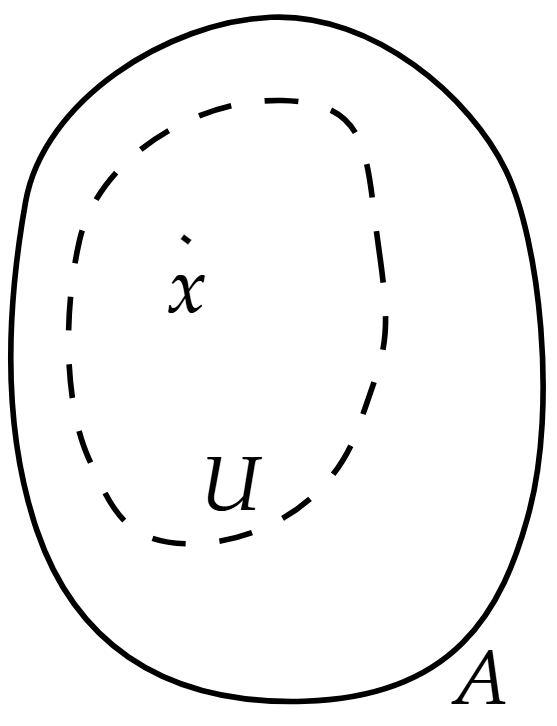
\includegraphics[width=0.12\textwidth]{fig/2.1.1.png}
    \vspace{-6 em}
\end{wrapfigure}
\begin{proof}
    “$\Rightarrow$” 显然成立.\par
    “$\Leftarrow$” $\forall\, x \in A,\exists\, x\text{的一个邻域}\,U_x,\st x\in U_x\subset A$，所以$A=\bigcup_{x\in A}{U_x}$.\par
    由于$U_x$是$X$的一个开集，所以$A$是一个开集.    
\end{proof}

\section{拓扑基}
\vspace{-1 em}
\begin{definition}{拓扑基}
    设$X$是一个集合，$\cal{B}$是$X$的子集族，若$\cal{B}$满足条件：
    \begin{enumerate}
        \item $\forall\, x\in X,\exists\, B\in\cal{B},\st x\in B,\ie X=\bigcup_{B\in\cal{B}}{B}$
        \item 若$B_1,B_2\in\cal{B},x\in B_1\cap B_2$，则$\exists\, B\in\cal{B},\st x\in B\subset B_1\cap B_2$
    \end{enumerate}
    则称$\cal{B}$为$X$的\textbf{拓扑基}.
\end{definition}
下图直观地展示了拓扑基的第二个条件.
\begin{figure}[h]
    \centering
    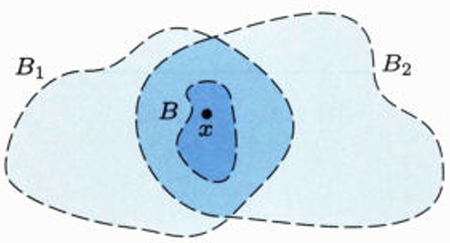
\includegraphics[width=0.5\textwidth]{fig/2.2.1.png}
    \captionof{figure}{拓扑基的特性}
\end{figure}

\begin{theorem}{拓扑基生成拓扑}
    设$\cal{B}$为$X$的拓扑基，$\cal{T}=\{\cal{B}\text{中任意多个子集的并}\}$，则$\cal{T}$是$X$上的拓扑，称其为由拓扑基$\cal{B}$生成的拓扑，$\cal{B}$中的子集称为\textbf{基元素}.
\end{theorem}

\begin{proof}
    \begin{enumerate}[label=(\roman*)]
        \item $\varnothing,X\in\cal{T}$
        \item 对任意并的封闭性显然
        \item $U_1=\bigcup_{\alpha}{B_\alpha},U_2=\bigcup_{\beta}{C_\beta},\; B_\alpha,C_\beta\in\cal{B}$，则$U_1\cap U_2=\bigcup_{\alpha,\beta}({B_\alpha\cap C_\beta})\in\cal{T}$.\par
        由条件2，$\forall\, x\in B_\alpha\cap C_\beta,\exists\, D_x\in \cal{B},\st x\in D_x\subset B_\alpha\cap C_\beta$.\par
        因此$B_\alpha\cap C_\beta = \bigcup_{x\in B_\alpha\cap C_\beta}{D_x} \xLongrightarrow{D_x\in\cal{T}} B_\alpha\cap C_\beta\in\cal{T}$.\par
        所以$U_1\cap U_2\in\cal{T}$.\par
    \end{enumerate}
\end{proof}


\begin{instance}
    在$\mathbb{R}_{std}$上，$\cal{B}=\{\mathbb{R}\text{中所有开区间}\}$，$\cal{B}$生成$\mathbb{R}_   {std}$.
\end{instance}

\begin{instance}
    $X\neq\varnothing,\cal{B}=\{\{x\}|x\in X\}$，$\cal{B}$生成$X$上离散拓扑.
\end{instance}

上述的$\cal{B}$一定是一个拓扑基，条件1显然，而$\cal{B}$中的所有元素都是单点集，因此交集为空，自然条件2成立.

\begin{instance}
    $\mathbb{R}$，$\cal{B}=\{\left[a,b\right)|a<b\}$是一个拓扑基，验证其确为一个拓扑基.\par
    \begin{enumerate}[leftmargin=3.75em]
        \item $\forall\, x\in\mathbb{R},x\in[x,x+1)\in \cal{B}$
        \item $[a,b)\cap[c,d) = [\max\{a,c\},\min\{c,d\})$.\par
        则$\forall\, x\in [a,b)\cap[c,d),x\in[\max\{a,c\},\min\{c,d\})$
    \end{enumerate}\par
    $\cal{B}$生成了$\mathbb{R}$上的拓扑，称为\bluebf{下极限拓扑}，记作$\mathbb{R}_l$.
\end{instance}


\begin{lemma}{拓扑基的等价刻画}
    假设$\cal{B}$是$X$中的子集族，如果$\cal{B}$满足：
    \begin{enumerate}
        \item $\forall\, x\in X,\exists\, B\in\cal{B},\st x\in B$.
        \item $B_1,B_2\in\cal{B}\Rightarrow B_1\cap B_2=\varnothing\,\text{或}\,B_1\cap B_2\in\cal{B}$
    \end{enumerate}
    则$\cal{B}$是$X$的拓扑基.
\end{lemma}
从上述引理中可以看出，相较于$X$上的拓扑，$X$上的拓扑基所满足的条件更加简单，它是更加规则的集合.

\begin{lemma}{开集的描述}
    设$X$是一个集合，$\cal{B}$是$X$上一个拓扑基，则$U\subset X$在由$\cal{B}$生成的拓扑中是开集当且仅当$\forall\, x\in U,\exists\, B_x\in\cal{B},\st x\in B_x\subset U$.
\end{lemma}
\begin{proof}
    “$\Rightarrow$” 根据定义，存在一组基元素$B_\lambda,\lambda\in\Lambda$，使得$U=\bigcup_{\lambda\in\Lambda}{B_\lambda}$.\par
    $\forall\, x\in U,x\in\bigcup_{\lambda\in\Lambda}{B_\lambda}\Rightarrow\exists\, \lambda \in \Lambda, \st x\in B_\lambda\subset U$.取$B_x=B_\lambda$即可.\par
    “$\Leftarrow$” 根据假设，$U=\bigcup_{x\in U}{B_x}$，$U$是一组基元素的并.因此$U$是开的.
\end{proof}


